\chapter{面向多节点单指标的异常检测算法}\label{chap:single_metric}

基于第二章揭示的多节点曲线相似性规律，本章开展面向单指标多节点场景的异常检测方法研究。首先，基于联通大数据生产环境构建高质量的单指标多节点时序数据集；其次，系统评估基于曲线相似性的多种检测方法在该数据集上的性能，并通过参数敏感性实验揭示阈值依赖性这一核心问题；在此基础上，提出I-SPOT自适应阈值算法，通过包容性数据池更新与周期性GPD重估机制消除人工调参需求；最后，将上述组件整合为统一的CSAD-AT（Curve Similarity-based Anomaly Detection with Adaptive Threshold）框架，融合多视角相似性评分、分数归一化聚合与自适应阈值检测，实现端到端的自适应异常检测。

\section{多节点单指标数据集构建}\label{sec:dataset}

本章研究的数据基础来源于真实的分布式集群生产环境，旨在构建能够反映集群节点协同行为、并包含明确异常标注的数据集，以支撑后续算法的训练、验证与对比分析。

\subsection{数据来源与采集}\label{subsec:data_source}

本研究的数据来源于中国联通大数据生产底座平台。该平台采用业界标准的YARN（Yet Another Resource Negotiator）架构进行分布式计算资源的统一调度与管理，其核心架构如图\ref{fig:yarn_arch}所示。ResourceManager作为集群的中央调度器，通过RPC Router接收各NodeManager的心跳与资源请求，并下发调度指令；各NodeManager负责本地容器的生命周期管理，通过RPC Client与ResourceManager保持持续通信；Prometheus监控系统实时采集各节点的运行指标并持久化存储。

\begin{figure}[htbp]
    \centering
    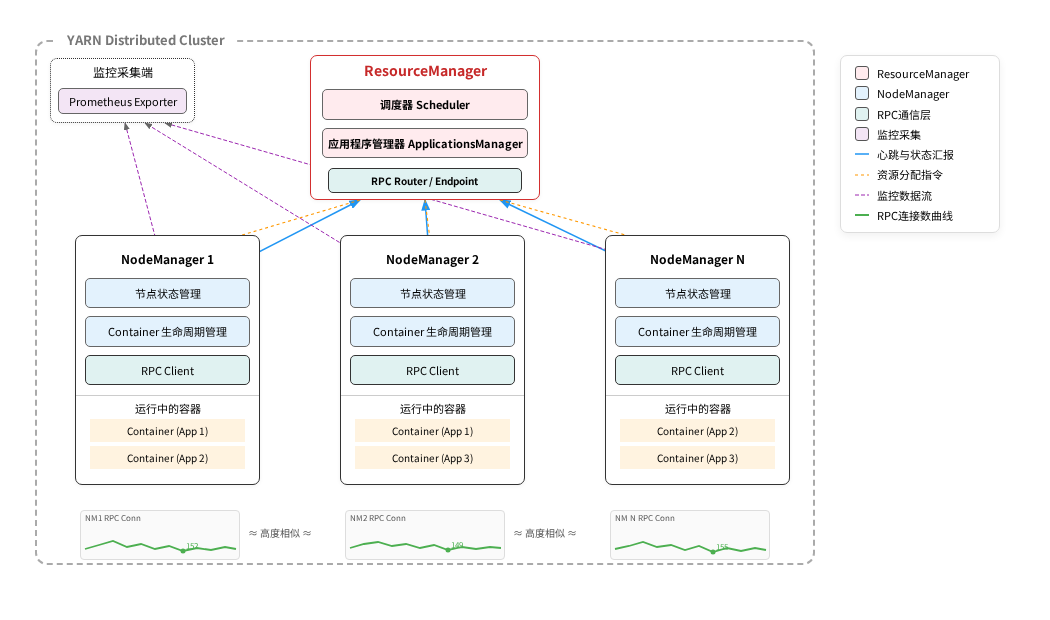
\includegraphics[width=0.85\textwidth]{Img/yarn_arch.png}
    \caption{YARN分布式集群架构与RPC Router连接数指标示意}
    \label{fig:yarn_arch}
\end{figure}

在长期运维实践中，我们观察到与用户负载强相关的监控指标（如RPC连接数）呈现出独特的统计特性：其正常波动模式难以通过先验知识统一定义，且随全局负载呈现不可预测的剧烈变化，导致传统基于绝对阈值或历史模式学习的方法面临高误报率。然而，得益于负载均衡机制的作用，正常运行状态下各节点同一指标的时序曲线呈现出高度的形态相似性（如图\ref{fig:yarn_arch}底部所示），这一规律性为基于"群体行为一致性"的异常检测提供了理论依据。

基于上述洞察，本研究选取RPC Router连接数作为核心研究指标。该指标直接反映各NodeManager与ResourceManager之间的通信负载与连接健康状态，是衡量节点服务能力的关键信号。本研究通过Prometheus API接口，采集了多个生产集群在连续运行周期内所有节点的该指标时序数据，形成训练集（覆盖30天连续运行数据）和测试集（覆盖8天连续运行数据），原始数据采样间隔为60秒。

\subsection{数据集预处理与标注}

为构建适用于算法研究的高质量数据集，并对后续模型性能进行可靠评估，本研究对从生产环境采集的原始监控时序数据实施了系统化的预处理流程，并采用了半人工标注策略。

原始监控数据在采集与传输过程中，可能因网络延迟、数据采集器（exporter）瞬时故障或系统抖动而产生缺失值。为确保时序数据的连续性，本研究采用线性插值法对短暂的数据缺失点进行填充。为确保不同节点间的时序曲线在时间维度上严格对齐，以进行有效的跨节点相似性比较，我们将所有数据点对齐至统一的60秒间隔时间戳上。此外，对于因监控代理长期离线、节点重启或下线等原因导致的长时间段数据完全缺失，线性插值将引入较大误差，针对此类情况，本研究直接剔除包含长时间段数据缺失的整条节点记录，以保证进入模型的数据的完整性与可靠性。

获得高质量的异常标注是进行模型评估和算法对比的基础。然而，生产环境中的异常样本缺乏记录，且缺乏自动化标注工具。本研究采用算法初步筛选与专家经验判读相结合的方式进行半人工标注，旨在确保标注结果的准确性。具体流程如图\ref{fig:annotation_flow}所示。

\begin{figure}[htbp]
    \centering
    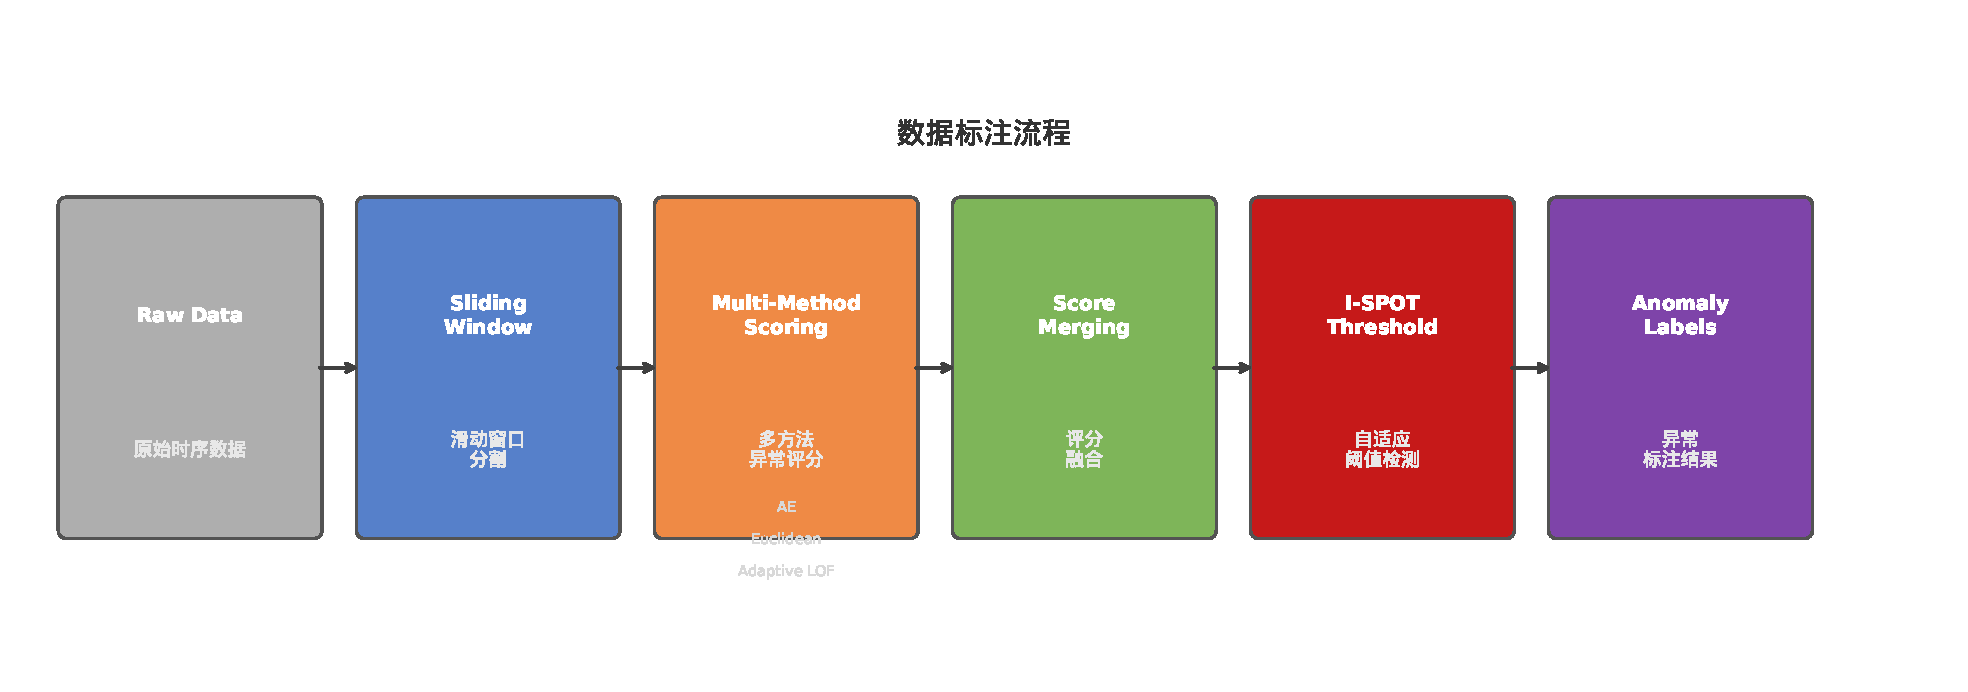
\includegraphics[width=0.85\textwidth]{Img/draft/annotation_flow.pdf}
    \caption{数据标注流程示意图}
    \label{fig:annotation_flow}
\end{figure}

首先，利用多种基础的无监督离群点检测算法对全体时序数据进行初步扫描，且将阈值设为宽松值，筛选出偏离其自身历史基线或群体平均模式的"疑似异常"时间片段。此步骤旨在缩小人工审查的范围，提升标注效率。

其次，对于初筛出的疑似异常片段，关联查询该时段内对应节点的运维数据，如日志、运维工单记录、相关指标时序数据等，对初步筛选出的异常点进行交叉验证，辅助判断其是否为真实的节点级故障或性能异常。

最终，由具备丰富分布式集群运维经验的专家，结合上一步的关联数据，并可视化审查疑似片段及其前后上下文的多节点曲线对比图，最终做出异常点判定。通过以上流程，对两个独立的YARN集群测试集进行了标注，形成了包含精确起止时间戳的异常片段集合。

\subsection{数据集统计与可视化}

经过预处理与标注，本研究构建了一个适用于分布式集群节点级异常检测研究的单指标多节点时间序列数据集。该数据集的详细统计信息如表\ref{tab:dataset_stats}所示。

\begin{table}[htbp]
    \centering
    \caption{数据集统计数据}
    \label{tab:dataset_stats}
    \begin{tabular}{lccccc}
        \hline
        & 节点数 & 数据点数量 & 异常片段数 & 异常点数量 & 异常比例 \\
        \hline
        训练集 & 30 & 86400 & / & / & / \\
        测试集A & 15 & 11520 & 72 & 901 & 7.82\% \\
        测试集B & 15 & 11520 & 33 & 907 & 7.87\% \\
        测试集 & 30 & 23040 & 105 & 1808 & 7.85\% \\
        \hline
    \end{tabular}
\end{table}

本数据集的核心特征在于其直观揭示了分布式集群在负载均衡机制下的运行规律，如图\ref{fig:anomaly_curve}所示。在绝大部分时间内，集群内多数节点的监控指标曲线呈现出高度的形态同步性与数值聚集性，它们紧密缠绕，形成清晰的"正常行为簇"。这反映了在系统负载均衡策略下，各节点承担相近的工作负载，行为模式高度一致。然而，当个别节点发生资源竞争、进程僵死、网络隔离或本地硬件故障等问题时，其监控曲线会显著偏离这个共同的"行为簇"，表现为形态各异、幅度不一的"离群曲线"。这种"正常聚集，异常离群"的鲜明数据特征，是本研究所提出的、基于群体相似性进行异常检测方法的依据与直观体现。

\begin{figure}[htbp]
    \centering
    % TODO: 插入测试数据集多节点曲线及异常标注示意图
    % \includegraphics[width=0.9\textwidth]{Img/anomaly_curve}
    \caption{测试数据集异常标注曲线（红色阴影部分为异常标注）}
    \label{fig:anomaly_curve}
\end{figure}

\section{现有异常检测方法评估}\label{sec:method_eval}

本节首先系统评估了一系列现有的时间序列异常检测算法在本研究构建的分布式集群数据集上的性能。\ref{subsec:baseline}节与\ref{subsec:similarity}节分别介绍了选择的先进的异常检测基线算法和基于曲线相似性的检测方法。在\ref{subsec:exp_results}节介绍了以上算法在分布式集群数据集上的实验结果。随后，\ref{subsec:param_sensitivity}节通过系统的参数敏感性实验揭示了这些方法在实际部署中面临的阈值依赖性和泛化能力不足等核心挑战，为后续自适应阈值算法的提出提供了直接动机。

\subsection{异常检测基线算法}\label{subsec:baseline}

为全面评估现有方法在分布式集群多节点场景下的适用性，本研究选取了六种具有代表性的先进异常检测算法作为基线，这些算法涵盖了基于重构、基于预测以及基于生成对抗网络等多种主流范式。

在基于重构的方法中，OmniAnomaly采用随机变分自编码器和平面归一化流来学习多元时间序列的正常模式分布，通过重构概率来识别异常样本。USAD则在自编码器架构的基础上引入对抗性训练机制，通过增强模型的鲁棒性来提升重构误差对异常的敏感性。

在基于预测的方法中，GDN通过图神经网络显式建模变量间的拓扑关系，利用对未来值的预测偏差来检测异常。TranAD基于Transformer架构构建深度异常检测模型，借助注意力机制捕捉序列中的长期依赖关系，并通过对抗训练增强对异常的敏感度。MTAD-GAT结合了图注意力网络和时间卷积网络，能够同时建模变量间的关联关系和时间维度的依赖模式。

在基于生成对抗网络的方法中，MAD-GAN采用LSTM构建生成器和判别器，通过对抗训练学习正常数据的分布特征，综合利用判别器得分和重构误差来识别异常。

实验设置遵循公平对比原则，所有基线模型均使用其作者开源的原版代码和默认推荐参数进行训练与测试。训练阶段使用\ref{subsec:data_source}节所述的同构集群30天正常数据，测试阶段在本研究标注的两个测试集上进行评估并报告合并测试集的整体性能。评估指标采用异常检测领域通用的精确率、召回率和F1分数。

\subsection{基于曲线相似性的异常检测方法}\label{subsec:similarity}

基于前文对分布式集群多节点行为一致性特征的分析，本节选取了三种基于曲线相似性的异常检测方法。这些方法的核心思想是通过度量节点间曲线的差异程度来识别偏离群体行为模式的异常节点，分别从数值距离、深度特征嵌入和局部密度三个不同角度刻画节点间的相似性关系。

\subsubsection{基于欧氏距离的数值相似性度量}

欧氏距离作为度量空间中最基本的距离度量方式，能够直接量化节点间曲线在数值空间中的差异程度。该方法具有计算简单、物理意义直观的优点，适用于对曲线数值偏离敏感的异常检测场景。

给定一个包含$N$个节点的分布式集群，每个节点$i$在时刻$t$的监控指标观测值记为$x_i^t$。为了捕捉时间序列的局部变化模式并降低瞬时噪声的影响，本方法采用滑动窗口机制对原始序列进行分段处理。对于长度为$w$的时间窗口，节点$i$在时刻$t$的窗口序列可表示为向量形式$\mathbf{x}_i^t = [x_i^{t-w+1}, x_i^{t-w+2}, \ldots, x_i^t]^T \in \mathbb{R}^w$。基于此，节点$i$与节点$j$在时刻$t$的欧氏距离定义为两个窗口向量之间的L2范数：

\begin{equation}
    d_{ij}^t = \|\mathbf{x}_i^t - \mathbf{x}_j^t\|_2 = \sqrt{\sum_{k=t-w+1}^{t}(x_i^k - x_j^k)^2}
\end{equation}

为了从多节点距离信息中识别异常节点，本方法设计了基于统计标准化的异常分数计算机制。首先，在时刻$t$的滑动窗口内计算所有节点两两之间的欧氏距离，构成距离矩阵$\mathbf{D}^t \in \mathbb{R}^{N \times N}$。然后，计算该距离矩阵中所有非对角元素的均值$\mu_t$和标准差$\sigma_t$，以此表征当前时刻整个集群的曲线整体相似性水平。对于每个节点$i$，计算其与其他所有节点的平均距离：

\begin{equation}
    \bar{d}_i^t = \frac{1}{N-1}\sum_{j=1, j \neq i}^{N} d_{ij}^t
\end{equation}

节点$i$在时刻$t$的异常分数采用Z-score标准化形式计算：

\begin{equation}\label{eq:euc_score}
    s_i^t = \frac{\bar{d}_i^t - \mu_t}{\sigma_t}
\end{equation}

该标准化过程将异常分数转换为相对于群体平均水平的偏离程度，消除了不同时刻集群整体负载水平差异带来的影响。在异常判定阶段，设定阈值$T$，若$s_i^t > T$，则判定节点$i$在时刻$t$发生异常。

欧氏距离方法的理论依据在于分布式集群的负载均衡特性。在系统正常运行时，负载均衡机制确保各节点承担相近的工作负载，因此正常节点的监控曲线应保持较高的相似性，其异常分数将聚集在较低水平。当某个节点发生故障或性能异常时，其曲线会显著偏离其他节点的共同模式，导致该节点与其他节点的平均距离增大，异常分数相应升高。

\subsubsection{基于自编码器嵌入的形态相似性度量}

欧氏距离方法对曲线的绝对数值高度敏感，可能忽略形态层面的相似性。例如，两条变化趋势相同但振幅不同的曲线，在欧氏距离度量下差异较大，但形态上实际高度一致。为克服这一局限，本研究引入自编码器进行深度特征提取，通过学习曲线形态的抽象表示来度量节点间相似性。

自编码器是一种无监督表示学习模型，由编码器$f_{\text{enc}}$和解码器$f_{\text{dec}}$组成。编码器将输入序列$\mathbf{x}_i^t$压缩为低维嵌入向量$\mathbf{z}_i^t = f_{\text{enc}}(\mathbf{x}_i^t)$，解码器从嵌入向量重构原始输入。通过最小化均方重构误差进行训练，自编码器能够在低维空间中保留曲线的本质形态特征，相比原始数值表示，嵌入向量对曲线的整体趋势、周期性和变化模式等形态特征更加敏感，而对绝对数值差异相对不敏感。

在应用阶段，使用编码器为各节点生成嵌入向量，后续基于嵌入向量计算节点间距离$d_{ij}^t = \|\mathbf{z}_i^t - \mathbf{z}_j^t\|_2$，异常分数计算流程与欧氏距离方法一致。本研究采用的自编码器网络结构包含三层全连接编码器（$60 \to 128 \to 128 \to 5$）和对称的三层解码器（$5 \to 128 \to 128 \to 60$），激活函数采用ReLU，优化器采用Adam，学习率设置为0.001，使用训练集数据训练50个epoch。

\subsubsection{基于DBSCAN聚类的密度相似性度量}\label{subsec:density_score}

除了基于距离度量的方法外，基于密度的聚类算法也能够有效识别偏离主流模式的异常点。DBSCAN算法是密度聚类的经典代表，其核心思想是将数据空间划分为高密度区域形成的簇和低密度区域中的离群点，具有无需预先指定簇数量、能够发现任意形状簇以及自动识别噪声点等优点。

DBSCAN算法基于两个关键参数进行聚类：邻域半径$\epsilon$和最小样本数$MinPts$。对于数据点$p$，其$\epsilon$邻域定义为$N_\epsilon(p) = \{q \in D \mid dist(p,q) \leq \epsilon\}$。若$|N_\epsilon(p)| \geq MinPts$，则$p$为核心点；若$p$不是核心点但位于某个核心点的$\epsilon$邻域内，则$p$为边界点；否则$p$为噪声点。算法通过密度可达关系将核心点及其密度相连的点聚合为簇，而噪声点则不属于任何簇。

在多节点异常检测场景中，本方法对每个时间窗口内的节点曲线进行DBSCAN聚类分析。具体而言，将节点$i$在时刻$t$的窗口序列$\mathbf{x}_i^t$作为特征向量，对所有$N$个节点的特征向量集合执行DBSCAN聚类。被算法标记为噪声点的节点即被判定为在该时刻发生异常。

该方法的检测逻辑与分布式集群的运行特性高度契合。在负载均衡机制的作用下，正常运行的节点其监控曲线形态相似，在特征空间中应当聚集形成高密度簇。而发生故障或性能异常的节点，其曲线会显著偏离主流模式，在特征空间中表现为远离高密度区域的孤立点，从而被DBSCAN算法自动识别为噪声。

DBSCAN方法的主要优势在于无需人工设定异常分数阈值，算法能够自适应地根据数据分布特征划分正常簇和异常点。然而，该方法对邻域半径$\epsilon$参数较为敏感，需要根据具体数据特征进行调优。

\subsection{实验结果对比分析}\label{subsec:exp_results}

为验证基于曲线相似性的异常检测方法的有效性，本节在构建的单指标多节点RPC连接数数据集上进行系统的对比实验。实验将上述三种方法与多种先进的多元时序异常检测算法进行比较，评估各方法在分布式集群场景下的检测性能。

实验结果如表\ref{tab:baseline_results}所示，表中上半部分为六种基线算法的检测结果，下半部分为三种基于曲线相似性方法的检测结果。

\begin{table}[htbp]
    \centering
    \caption{基线算法与曲线相似性方法在RPC Router连接数数据集上的异常检测效果对比}
    \label{tab:baseline_results}
    \begin{tabular}{lccc}
        \hline
        算法 & Precision & Recall & F1 \\
        \hline
        TranAD & 0.8889 & 0.3932 & 0.5452 \\
        USAD & 0.6892 & 0.5567 & 0.6159 \\
        OmniAnomaly & 0.6054 & 0.4593 & 0.5224 \\
        GDN & 0.3101 & 0.5218 & 0.3890 \\
        MAD\_GAN & 0.6309 & 0.6309 & 0.6891 \\
        MTAD\_GAT & 0.3492 & 0.1573 & 0.2169 \\
        \hline
        欧氏距离 & 0.9826 & 0.9657 & 0.9741 \\
        自编码器嵌入 & 0.9792 & 0.9592 & 0.9691 \\
        密度偏离 & 0.9605 & 0.9659 & 0.9632 \\
        \hline
    \end{tabular}
\end{table}

从实验结果可以观察到，现有的多元时序异常检测算法在本数据集上的表现普遍欠佳。具体而言，TranAD虽然取得了较高的精确率（0.8889），但召回率仅为0.3932，表明该方法遗漏了大量真实异常。USAD和OmniAnomaly作为基于重构的方法，在精确率和召回率之间取得了相对均衡的结果，但F1分数均未超过0.65。GDN和MTAD-GAT作为基于图神经网络的方法，在该数据集上的表现最差，这可能是因为这些方法主要针对多变量间的关联异常设计，而本数据集的异常主要表现为单节点的行为偏离。MAD-GAN在基线方法中表现相对最好，但F1分数也仅为0.6891。

分析基线算法表现不佳的原因，主要在于负载均衡类指标的固有特性。此类指标的正常波动具有随机性和不可预测性，难以通过历史数据学习出稳定的正常模式。基于重构或预测的深度学习方法往往只能学习到数据的主要趋势，对于负载突变和大幅波动容易产生误报，而对于相对于其他节点偏离但绝对值在正常范围内的异常则容易漏报。

相比之下，三种基于曲线相似性的方法均取得了显著更优的检测效果。欧氏距离方法在最优参数配置下达到了0.9741的F1分数，精确率和召回率分别为0.9826和0.9657。自编码器嵌入方法取得了0.9691的F1分数，密度偏离方法取得了0.9632的F1分数。三种方法的F1分数均超过0.96，显著优于所有基线算法。

这一结果充分验证了基于多节点曲线相似性进行异常检测的核心思路的有效性。通过对比节点间的曲线差异而非学习绝对的正常模式，本方法能够有效规避负载敏感型指标波动性强带来的挑战。然而，实验也发现三种方法的性能对参数选择较为敏感。欧氏距离和自编码器嵌入方法需要设定合适的异常分数阈值，密度偏离方法同样需要调整相关参数。阈值或参数设置的细微偏差可能导致检测效果急剧下降。针对这一问题，下一小节将详细介绍参数敏感性实验分析。

\subsection{阈值敏感性实验与分析}\label{subsec:param_sensitivity}

前文提出的三种基于曲线相似性的异常检测方法均涉及关键超参数的设定，这些参数直接影响检测性能的优劣。为深入理解参数选择对算法表现的影响规律，本节在构建的单指标多节点数据集上开展系统的参数敏感性实验，分别考察时间窗口大小和检测阈值两个维度对三种方法检测效果的影响，实验结果如表\ref{tab:euclidean_sensitivity}、表\ref{tab:ae_sensitivity}和表\ref{tab:density_sensitivity}所示。

\begin{table}[htbp]
    \centering
    \caption{欧氏距离方法在不同阈值和时间窗口下的异常检测分数}
    \label{tab:euclidean_sensitivity}
    \resizebox{\textwidth}{!}{
    \begin{tabular}{l|ccc|ccc|ccc}
        \hline
        & \multicolumn{3}{c|}{window size=10} & \multicolumn{3}{c|}{window size=20} & \multicolumn{3}{c}{window size=30} \\
        threshold & Precision & Recall & F1 & Precision & Recall & F1 & Precision & Recall & F1 \\
        \hline
        3.0 & 0.5485 & 1.0000 & 0.7084 & 0.7251 & 1.0000 & 0.8406 & 0.8214 & 1.0000 & 0.9020 \\
        3.2 & 0.6797 & 1.0000 & 0.8093 & 0.7892 & 1.0000 & 0.8822 & 0.8593 & 1.0000 & 0.9243 \\
        3.4 & 0.8116 & 1.0000 & 0.8960 & 0.8974 & 1.0000 & 0.9459 & 0.9256 & 1.0000 & 0.9614 \\
        3.6 & 0.9532 & 0.9655 & 0.9593 & 0.9826 & 0.9657 & 0.9741 & 0.9727 & 0.9469 & 0.9596 \\
        3.7 & 0.9946 & 0.9242 & 0.9581 & 0.9928 & 0.8839 & 0.9352 & 0.9944 & 0.8856 & 0.9368 \\
        3.8 & 0.0000 & 0.0000 & 0.0000 & 0.0000 & 0.0000 & 0.0000 & 0.0000 & 0.0000 & 0.0000 \\
        \hline
    \end{tabular}
    }
\end{table}

\begin{table}[htbp]
    \centering
    \caption{自编码器嵌入方法在不同阈值和时间窗口下的异常检测分数}
    \label{tab:ae_sensitivity}
    \resizebox{\textwidth}{!}{
    \begin{tabular}{l|ccc|ccc|ccc}
        \hline
        & \multicolumn{3}{c|}{window size=10} & \multicolumn{3}{c|}{window size=20} & \multicolumn{3}{c}{window size=30} \\
        threshold & Precision & Recall & F1 & Precision & Recall & F1 & Precision & Recall & F1 \\
        \hline
        3.0 & 0.4370 & 0.9833 & 0.6051 & 0.6028 & 1.0000 & 0.7522 & 0.7206 & 1.0000 & 0.8376 \\
        3.6 & 0.9507 & 0.8977 & 0.9234 & 0.9793 & 0.9404 & 0.9595 & 0.9792 & 0.9592 & 0.9691 \\
        3.8 & 0.0000 & 0.0000 & 0.0000 & 0.0000 & 0.0000 & 0.0000 & 0.0000 & 0.0000 & 0.0000 \\
        \hline
    \end{tabular}
    }
\end{table}

\begin{table}[htbp]
    \centering
    \caption{密度偏离方法在不同参数下的异常检测分数}
    \label{tab:density_sensitivity}
    \begin{tabular}{lccc}
        \hline
        参数设置 & Precision & Recall & F1 \\
        \hline
        eps=200 & 0.0332 & 1.0000 & 0.0642 \\
        eps=300 & 0.3442 & 1.0000 & 0.5121 \\
        eps=400 & 0.8302 & 1.0000 & 0.9072 \\
        eps=500 & 0.9605 & 0.9659 & 0.9632 \\
        \hline
    \end{tabular}
\end{table}

从实验结果可以观察到以下规律。在时间窗口维度上，三种方法均表现出窗口越大、检测效果越稳定的趋势。以欧氏距离方法为例，在阈值为3.4时，窗口大小从10增加到30，F1分数从0.8960提升至0.9614。这一现象的原因在于较大的时间窗口能够包含更丰富的时序模式信息，有效平滑瞬时噪声的干扰，使得节点间的相似性度量更加稳健。然而，窗口过大也会导致检测延迟增加，在实际应用中需要在检测精度和响应速度之间进行权衡。

在阈值维度上，三种方法均呈现出典型的精确率与召回率此消彼长的特征。当阈值设置偏低时，算法倾向于将更多的样本判定为异常，导致召回率较高但精确率下降，产生较多误报。当阈值设置偏高时，只有偏离程度极大的样本才会被判定为异常，精确率提高但召回率下降，导致部分真实异常被遗漏。

实验结果进一步揭示了各方法对阈值选择的高度敏感性。以欧氏距离方法为例，当阈值从最优值3.6略微调整至3.7时，召回率便从0.9657骤降至0.8839，而阈值升至3.8时检测完全失效。自编码器嵌入方法表现出类似的敏感特性，最优阈值同样处于一个狭窄的区间内。密度偏离方法的参数同样对检测效果影响显著，参数变化导致F1分数从0.0642跃升至0.9632，表明参数选择不当会使算法性能产生数量级的差异。

\subsection{参数依赖性与泛化挑战}

上述敏感性实验结果揭示了基于曲线相似性的异常检测方法在实际部署中面临的核心挑战。尽管三种方法在最优参数配置下均能取得优异的检测效果，但这种高性能严重依赖于精确的参数调优，而参数调优过程本身又依赖于充足的标注数据，形成了方法实用化的主要障碍。

从参数依赖性的角度分析，三种方法的最优参数均处于一个狭窄的有效区间内，超出该区间后性能急剧下降。这种"悬崖效应"的根源在于异常检测任务本身的特殊性：异常样本在总体样本中占比极低，导致精确率和召回率对决策边界的位置高度敏感。以欧氏距离方法为例，阈值从3.6调整到3.7仅变化约2.8\%，但F1分数却下降了约4\%，这种非线性的性能衰减特性给参数选择带来了极大的困难。

从泛化能力的角度分析，最优参数的确定严重依赖于特定数据集的统计特性。不同集群的节点数量、负载模式、监控指标量纲等因素均会影响曲线相似性的分布特征，进而改变最优阈值的位置。在一个集群上调优得到的参数，直接迁移到另一个集群往往难以取得理想效果。这种泛化性不足的问题限制了方法的可扩展性，难以满足大规模分布式系统中多集群统一监控的实际需求。

从工程实践的角度分析，生产环境中获取高质量标注数据的成本极高。异常事件本身具有稀疏性和多样性的特点，完整覆盖各类异常模式需要长期积累。同时，异常标注需要具备领域专业知识的运维人员进行判断，人力成本高昂。更为关键的是，系统运行环境会随时间演化，历史数据上调优的参数可能因概念漂移而逐渐失效，需要持续的人工干预和重新标定。

综合以上分析，如何降低算法对预设阈值的依赖性，实现阈值的动态自适应调整，成为将基于曲线相似性的异常检测方法推向实际生产应用的关键技术挑战。针对这一问题，下一节将引入基于极值理论的自适应阈值算法。

\section{I-SPOT包容性自适应阈值算法}\label{sec:threshold}

上一节的实验表明，基于曲线相似性的异常检测方法虽然在最优参数下取得了优异的性能，但对阈值选择高度敏感，难以在实际部署中推广。为解决这一问题，本节引入基于极值理论（Extreme Value Theory, EVT）的自适应阈值方法，首先介绍经典SPOT算法的原理及其局限性，随后提出改进的I-SPOT算法。

\subsection{SPOT算法原理}

SPOT（Streaming Peaks Over Threshold）算法的核心思想是利用广义帕累托分布（Generalized Pareto Distribution, GPD）对数据分布的尾部进行建模，从而在无需预先假设数据整体分布形式的情况下，自动确定异常判定的阈值边界。

给定异常分数序列$\{s_1, s_2, \ldots, s_n\}$，SPOT算法首先选取一个初始阈值$t_0$（通常取序列的高分位数），将超过该阈值的观测值称为"超额"（exceedance）。根据极值理论中的Pickands-Balkema-de Haan定理，当初始阈值$t_0$足够高时，超额值$Y = S - t_0$（其中$S > t_0$）的条件分布可以用GPD来近似：
\begin{equation}
    G_{\xi,\sigma}(y) = 1 - \left(1 + \frac{\xi y}{\sigma}\right)^{-1/\xi}, \quad y > 0
\end{equation}
其中$\xi$为形状参数，$\sigma > 0$为尺度参数。通过Grimshaw方法对超额值序列进行极大似然估计，可以得到参数$\hat{\xi}$和$\hat{\sigma}$的估计值。进而，对于给定的风险水平$q$，异常检测阈值可计算为：
\begin{equation}\label{eq:spot_threshold}
    z_q = t_0 + \frac{\hat{\sigma}}{\hat{\xi}}\left[\left(\frac{n}{N_t} \cdot q\right)^{-\hat{\xi}} - 1\right]
\end{equation}
其中$n$为总观测数，$N_t$为超过初始阈值$t_0$的观测数。

经典SPOT算法在流数据场景下持续更新GPD模型参数以适应数据分布的动态变化。然而，该算法在更新模型时仅将未超过阈值$z_q$的正常数据点纳入更新池，将判定为异常的数据点排除在外。这一设计在概念漂移场景下会引发阈值衰减问题：当正常数据的整体分布随时间缓慢上移时，越来越多的正常点被误判为异常而排除在模型更新之外，导致训练数据池被"截断"，基于截断样本估计的GPD参数使新阈值进一步降低，形成自我强化的误报螺旋。

\subsection{I-SPOT：包容性自适应阈值算法}

针对经典SPOT算法的阈值衰减问题，本研究提出I-SPOT（Inclusive SPOT）算法。其核心改进在于采用包容性更新策略：所有数据点（无论是否超过当前阈值）均纳入数据池，从而使模型能够动态跟踪数据分布的演化趋势。

I-SPOT算法维护一个最大容量为$W_{\max}$的先进先出（FIFO）数据池$\mathcal{D}_t$。对于每个新到达的异常分数$s_t$，更新规则定义为：
\begin{equation}
    \mathcal{D}_{t+1} = \begin{cases}
        \mathcal{D}_t \cup \{s_t\}, & \text{if } |\mathcal{D}_t| < W_{\max} \\
        (\mathcal{D}_t \setminus \{s_{\text{oldest}}\}) \cup \{s_t\}, & \text{otherwise}
    \end{cases}
\end{equation}
与经典SPOT不同，I-SPOT不对$s_t$是否超过阈值进行区分，所有观测值均被纳入后续的模型拟合过程。

在阈值更新方面，I-SPOT采用周期性重估策略：每隔$T_{\text{update}}$个时间步，基于当前数据池$\mathcal{D}_t$重新计算初始阈值$t_0^{(t)} = \text{Percentile}(\mathcal{D}_t, \text{level})$，提取超额量$Y = \{s - t_0^{(t)} \mid s \in \mathcal{D}_t, s > t_0^{(t)}\}$，通过Grimshaw方法重新拟合GPD参数$(\hat{\xi}^{(t)}, \hat{\sigma}^{(t)})$，并按式\eqref{eq:spot_threshold}更新自适应阈值$z_q$。

此外，I-SPOT引入自适应重置机制：当累计异常数或已处理数据点数达到预设阈值时，触发数据池的完全重置，以应对突发性的分布变化。I-SPOT算法的完整流程如算法\ref{alg:ispot}所示。

\begin{algorithm}[htbp]
    \caption{I-SPOT自适应阈值算法}
    \label{alg:ispot}
    \begin{algorithmic}[1]
        \Require 异常分数流 $\{s_1, s_2, \ldots\}$，风险水平 $q$，分位数水平 $\textit{level}$，数据池容量 $W_{\max}$，重估间隔 $T_{\text{update}}$，初始长度 $n_0$
        \Ensure 异常判定结果，动态阈值序列 $\{z_q^{(t)}\}$
        \State $\mathcal{D} \gets \{s_1, \ldots, s_{n_0}\}$；$t_0 \gets \text{Percentile}(\mathcal{D}, \textit{level})$ \Comment{初始化}
        \State $(\hat{\xi}, \hat{\sigma}) \gets \text{GrimshawMLE}(\{s - t_0 \mid s \in \mathcal{D},\, s > t_0\})$ \Comment{拟合GPD}
        \State $z_q \gets \text{ComputeThreshold}(t_0, \hat{\xi}, \hat{\sigma}, q)$；$\textit{steps} \gets 0$
        \For{\textbf{each} incoming score $s_t$}
            \If{$s_t > z_q$} 标记时刻 $t$ 为异常 \EndIf
            \If{$|\mathcal{D}| \geq W_{\max}$} $\mathcal{D} \gets \mathcal{D} \setminus \{s_{\text{oldest}}\}$ \EndIf \Comment{淘汰最旧}
            \State $\mathcal{D} \gets \mathcal{D} \cup \{s_t\}$；$\textit{steps} \gets \textit{steps} + 1$ \Comment{包容性更新}
            \If{$\textit{steps} \geq T_{\text{update}}$} \Comment{周期性重估}
                \State $t_0 \gets \text{Percentile}(\mathcal{D}, \textit{level})$
                \State $(\hat{\xi}, \hat{\sigma}) \gets \text{GrimshawMLE}(\{s - t_0 \mid s \in \mathcal{D},\, s > t_0\})$
                \State $z_q \gets \text{ComputeThreshold}(t_0, \hat{\xi}, \hat{\sigma}, q)$；$\textit{steps} \gets 0$
            \EndIf
        \EndFor
    \end{algorithmic}
\end{algorithm}

通过包容性更新策略，I-SPOT能够在保持对真实异常敏感性的同时，自适应地跟踪正常数据分布的长期演化趋势。当系统负载整体上升导致异常分数分布右移时，I-SPOT的阈值会相应上调，避免产生大量误报；当系统恢复稳定状态时，阈值又会逐渐回落至合适水平。

% TODO: 插入I-SPOT与经典SPOT阈值跟踪对比图
%\begin{figure}[htbp]
%    \centering
%    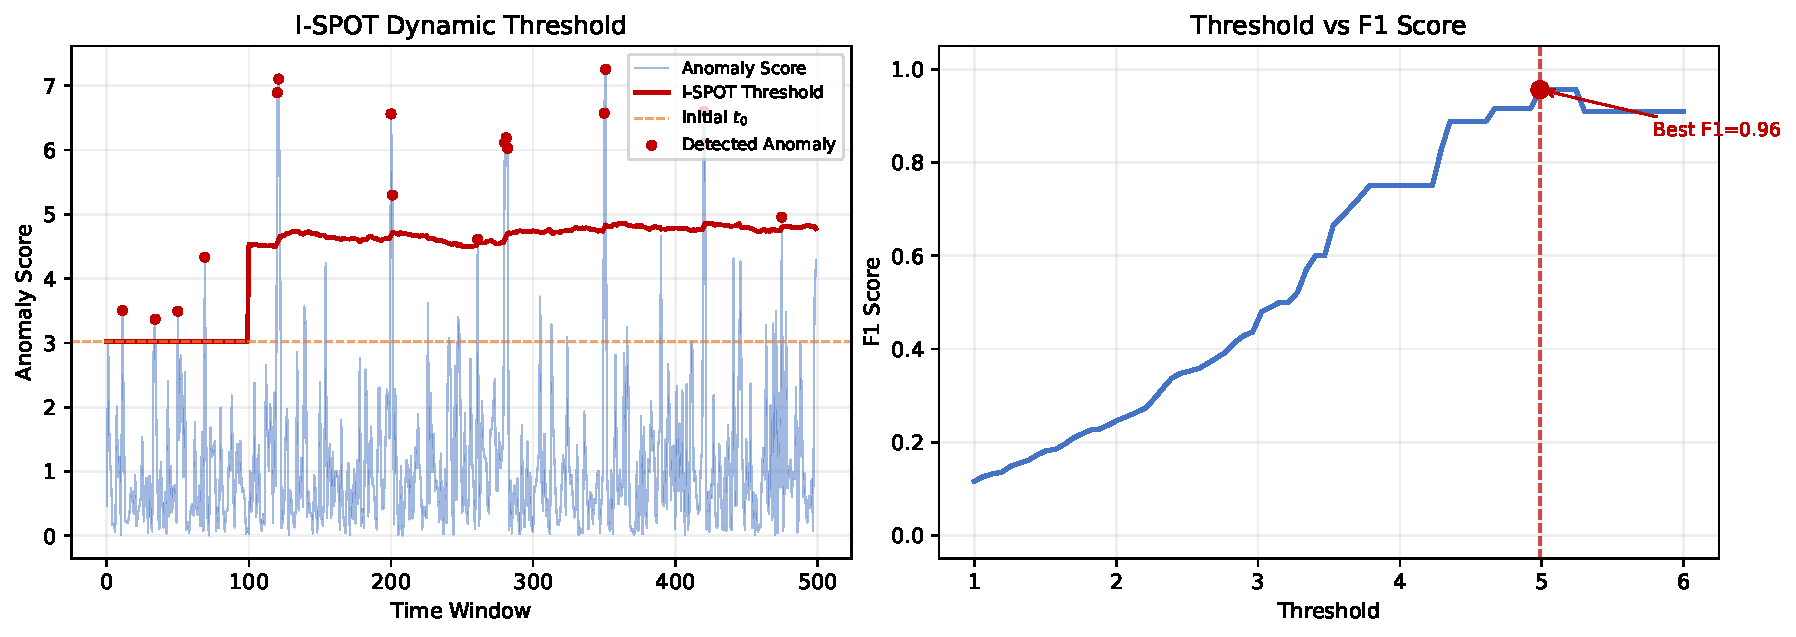
\includegraphics[width=0.85\textwidth]{Img/draft/threshold_f1.pdf}
%    \caption{I-SPOT与经典SPOT阈值跟踪对比}
%    \label{fig:threshold_compare}
%\end{figure}

\section{CSAD-AT异常检测框架}\label{sec:framework}

前两节分别评估了基于曲线相似性的异常评分方法的有效性，并提出了I-SPOT自适应阈值算法。本节将这些组件整合为统一的CSAD-AT（Curve Similarity-based Anomaly Detection with Adaptive Threshold）框架，通过异常评分、分数归一化与聚合、以及I-SPOT自适应阈值检测三个核心环节，实现端到端的自适应异常检测。

\subsection{框架概述}

CSAD-AT框架的整体架构如图\ref{fig:csad_framework}所示，包含三个核心模块：多视角相似性评分模块、分数归一化与聚合模块和I-SPOT自适应阈值检测模块。

\begin{figure}[htbp]
    \centering
    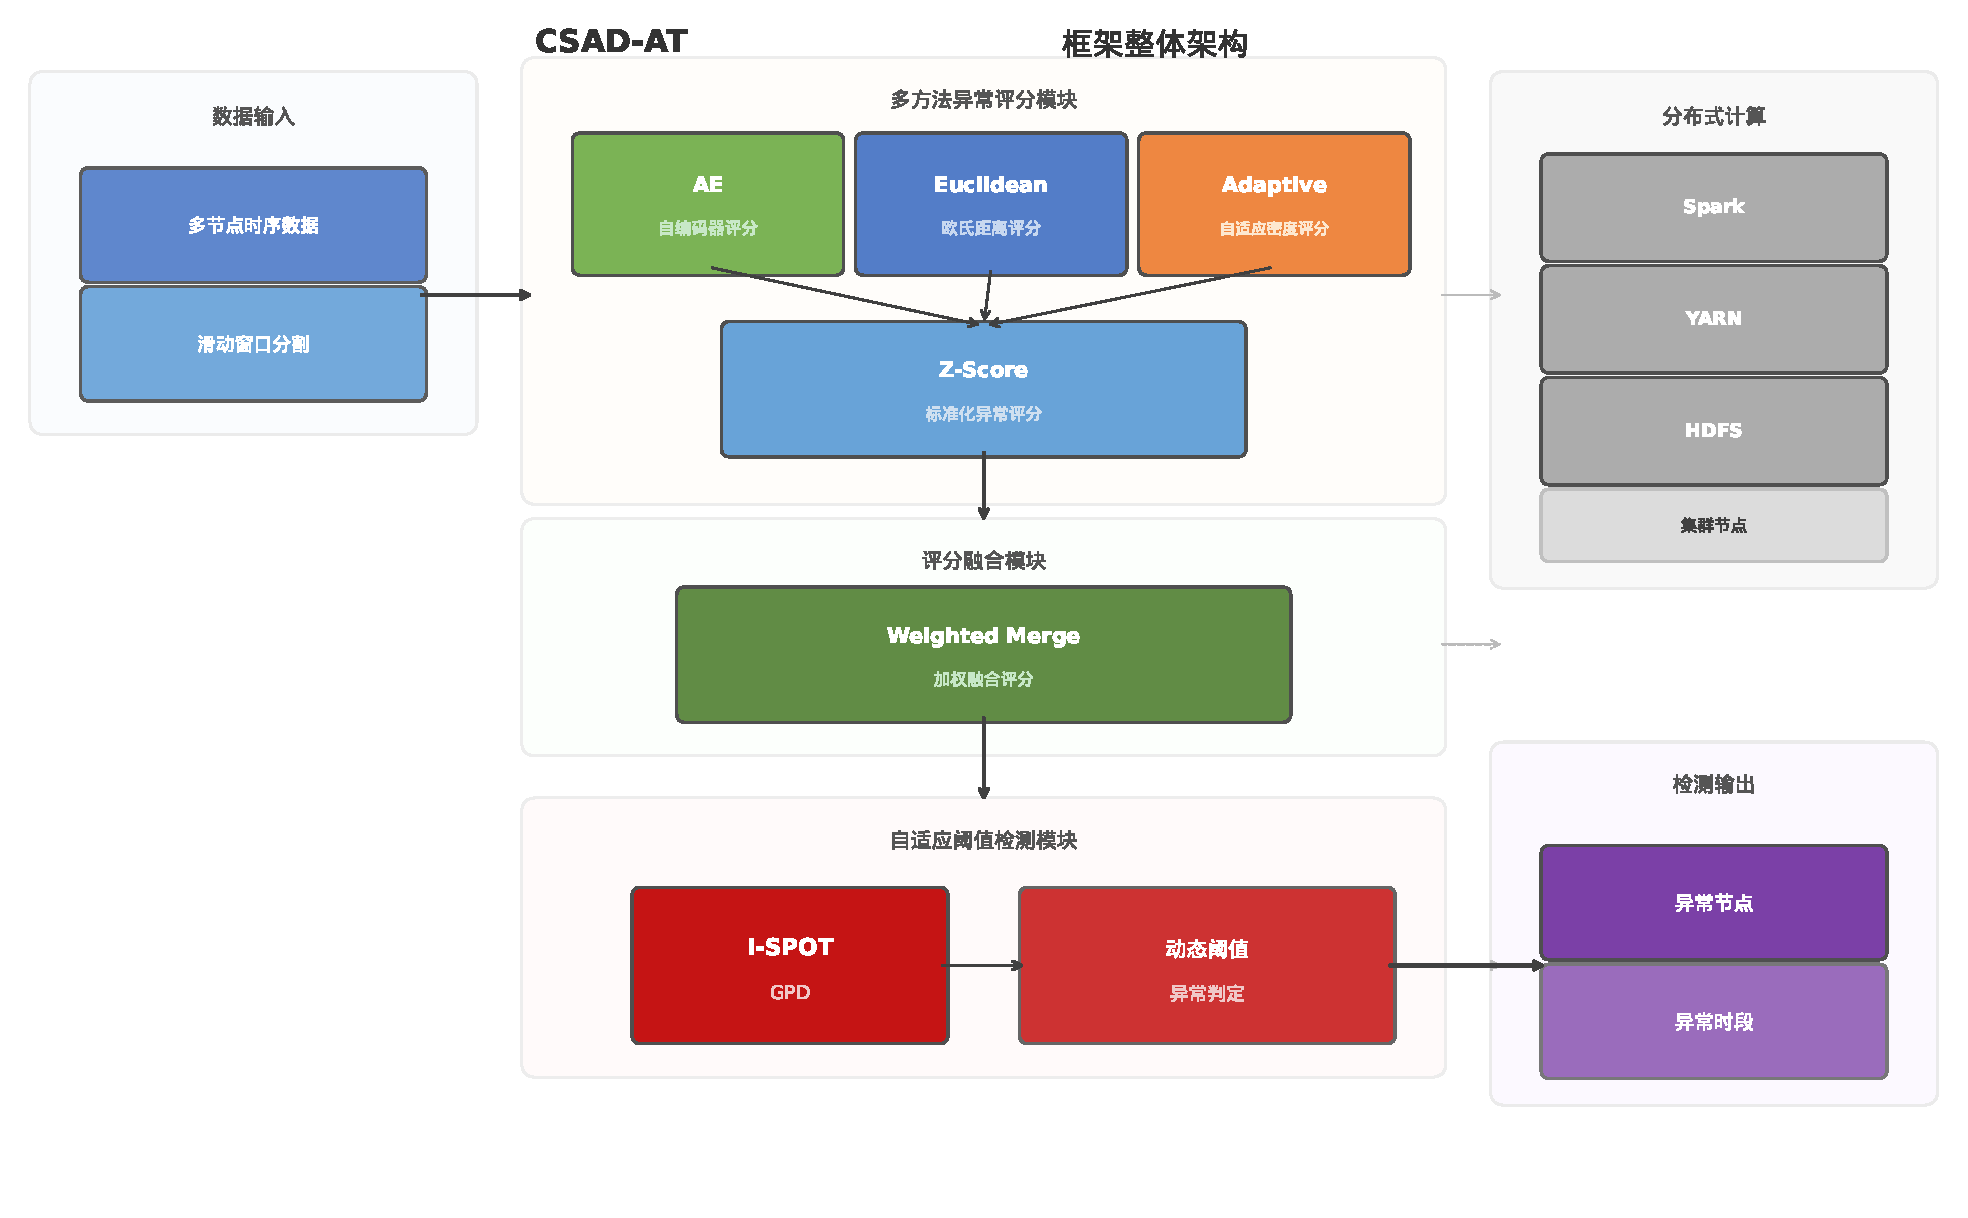
\includegraphics[width=0.9\textwidth]{Img/draft/csad_framework.pdf}
    \caption{CSAD-AT框架整体架构}
    \label{fig:csad_framework}
\end{figure}

框架的设计遵循三个原则：（1）互补视角：通过融合数值距离、嵌入空间距离和局部密度三种评分方法，提升对不同类型异常的覆盖能力；（2）分数归一化保证可比性：三种方法输出的原始分数量纲和范围不同，需经过统一的归一化处理后才能有效聚合；（3）统一全局阈值：将所有节点的聚合分数按时间窗口交织为全局序列，在全局序列上运行单一的I-SPOT实例，避免为每个节点单独维护阈值。

\subsection{异常评分方法}

CSAD-AT框架采用三种基于曲线相似性的异常评分方法，分别从数值距离、嵌入空间距离和局部密度三个互补视角对节点的偏离程度进行量化。三种方法均基于\ref{subsec:similarity}节所述的滑动窗口框架提取节点特征，并在此基础上计算异常分数。

\subsubsection{欧氏距离评分与自编码器嵌入评分}

欧氏距离评分直接度量原始窗口向量间的数值差异，对数值幅度偏离最为敏感。对于节点$i$在窗口$t$中的异常分数，按照\ref{subsec:similarity}节所述流程，先计算节点与其他所有节点的欧氏距离均值$\bar{d}_i^t$，再通过Z-score标准化得到异常分数$s_i^t = (\bar{d}_i^t - \mu_t) / \sigma_t$，其中$\mu_t$和$\sigma_t$分别为当前窗口内所有节点平均距离的均值和标准差。

自编码器嵌入评分则通过编码器将窗口序列映射到低维潜在空间，在潜在空间中度量形态差异，对曲线趋势和变化模式的偏离更加敏感。编码器将输入窗口序列压缩为低维嵌入向量，后续基于嵌入向量计算节点间距离，异常分数计算流程与欧氏距离方法一致。

\subsubsection{密度偏离评分}

与\ref{subsec:density_score}节介绍的DBSCAN聚类方法不同，CSAD-AT框架中的密度评分方法借鉴局部离群因子（Local Outlier Factor, LOF）的思想，设计了基于$k$近邻可达密度的连续异常评分方法。该方法不进行显式的簇划分，不依赖$\epsilon$邻域半径和$MinPts$等聚类参数，而是输出连续的异常分数，更适合与后续的归一化聚合及I-SPOT自适应阈值算法衔接。

对于每个时间窗口内的每个节点$i$，首先基于距离矩阵找到其$k_{\text{nn}}$个最近邻节点，记第$k_{\text{nn}}$近邻距离为$d_i^{k_{\text{nn}}}$。以$d_i^{k_{\text{nn}}}$作为自适应邻域半径，计算节点$i$的邻域集合$\mathcal{N}_i = \{j : d_{ij} \leq d_i^{k_{\text{nn}}}, j \neq i\}$。基于邻域信息，计算节点$i$的局部可达密度（Local Reachability Density, LRD）：
\begin{equation}
    \text{LRD}_i = \frac{1}{\frac{1}{|\mathcal{N}_i|}\sum_{j \in \mathcal{N}_i} d_{ij} + \epsilon}
\end{equation}
其中$\epsilon$为防止除零的小常数。LRD越高，表明节点$i$周围的邻居越密集，处于高密度区域。

为综合刻画节点的局部密度特征，本方法计算三个子分数的Z-score标准化值：（1）LRD的Z-score $z_{\text{LRD}}$；（2）第$k_{\text{nn}}$近邻距离的Z-score $z_{k\text{th}}$；（3）邻域内邻居数量的Z-score $z_{\text{nbr}}$。最终的密度偏离分数通过加权组合得到：
\begin{equation}\label{eq:density_score}
    s_i^t = w_1 \cdot z_{\text{LRD}} + w_2 \cdot z_{k\text{th}} + w_3 \cdot z_{\text{nbr}}
\end{equation}
其中权重的设计逻辑是：异常节点通常具有较低的局部密度（LRD偏低，故$w_1$取负值）、较大的$k$近邻距离（$z_{k\text{th}}$偏高，$w_2$取正值）以及较少的邻居（$z_{\text{nbr}}$偏低，$w_3$取负值）。加权组合后的分数再经过整体Z-score标准化，确保不同窗口间的分数具有可比性。

\subsubsection{多视角互补性}

三种方法形成有效的互补：欧氏距离捕捉数值突变型异常，自编码器嵌入识别形态模式异常，密度偏离发现局部孤立型异常。这种多视角的设计使得CSAD-AT框架能够覆盖更广泛的异常类型。

\subsection{分数归一化与聚合}

三种评分方法输出的原始异常分数在量纲和数值范围上存在显著差异，直接聚合将导致某些方法的贡献被掩盖。为此，CSAD-AT框架对每种方法的分数序列分别执行两步归一化处理。

第一步，负值截断：由于异常分数的正值表示偏离群体（潜在异常），负值表示与群体高度一致（正常），将所有负值截断为零：
\begin{equation}
    s'^{(m)} = \max(s^{(m)}, 0)
\end{equation}

第二步，MinMax归一化：将截断后的分数映射到$[0, 1]$区间：
\begin{equation}
    \tilde{s}^{(m)} = \frac{s'^{(m)} - s'^{(m)}_{\min}}{s'^{(m)}_{\max} - s'^{(m)}_{\min}}
\end{equation}
其中$s'^{(m)}_{\min}$和$s'^{(m)}_{\max}$分别为第$m$种方法截断后分数的最小值和最大值。经过归一化处理，三种方法的分数均位于$[0, 1]$区间内，具有统一的可比性。

归一化后的三种分数通过加权平均进行聚合，得到最终的综合异常分数：
\begin{equation}
    s_{\text{fused}} = \sum_{m=1}^{M} w_m \cdot \tilde{s}^{(m)}, \quad \sum_{m=1}^{M} w_m = 1
\end{equation}
其中$M=3$为评分方法数量，$w_m$为各方法的权重。默认采用等权设置$w_1 = w_2 = w_3 = 1/3$，即假设三种方法具有同等重要性。

选择加权平均作为聚合策略的理由在于：（1）相比最大值融合，加权平均保留了连续的分数信息，不会因单个方法的偶然高分而过度放大噪声；（2）相比投票机制，加权平均输出连续值，有利于后续I-SPOT的GPD尾部建模；（3）加权平均的计算开销极低，适合在线流式处理场景。实验中还对比了其他聚合策略，详见\ref{subsec:agg_compare}节。

\subsection{全局时间线构建与I-SPOT检测}

CSAD-AT框架的一个关键设计是将所有节点的聚合分数按窗口交织为全局时间序列，而非为每个节点独立运行阈值检测。具体而言，对于窗口$k$中$N$个节点的聚合分数$\{s_{\text{fused},0}^{(k)}, s_{\text{fused},1}^{(k)}, \ldots, s_{\text{fused},N-1}^{(k)}\}$，全局序列的排列方式为：
\begin{equation}
    \mathbf{S}_{\text{global}} = [s_{\text{fused},0}^{(0)}, s_{\text{fused},1}^{(0)}, \ldots, s_{\text{fused},N-1}^{(0)}, s_{\text{fused},0}^{(1)}, \ldots]
\end{equation}
即采用窗口优先、节点次序的交织方式。

在全局序列$\mathbf{S}_{\text{global}}$上运行I-SPOT算法，得到每个位置的异常判定结果。随后，将异常标记映射回（窗口，节点）矩阵，即可确定具体在哪个时间窗口的哪个节点发生了异常。

这种全局时间线设计的优势在于：（1）所有节点共享同一个I-SPOT实例和阈值，大幅降低了计算和存储开销；（2）全局序列的样本量更大，使GPD拟合更加稳健；（3）阈值能够同时反映所有节点的分数分布特征，对整体负载变化更加敏感。

\section{实验验证与分析}\label{sec:experiments}

\subsection{实验设置}

本节实验在本文构建的单指标多节点数据集上进行，旨在全面验证CSAD-AT框架及其各组件的有效性。实验环境采用配备Intel Core i7处理器和16GB内存的服务器，算法实现基于Python 3.8和相关科学计算库。

实验评估采用异常检测领域通用的精确率（Precision）、召回率（Recall）和F1分数三个指标。异常判定采用窗口级别的评估协议：若检测到的异常窗口与真实异常标注窗口的重叠比例超过50\%，则视为正确检测（True Positive）。

I-SPOT算法的超参数设置为：风险水平$q = 0.0085$，分位数水平$\text{level} = 0.98$，重估间隔$T_{\text{update}} = 50$，初始序列长度$n_0 = 1500$。

实验对比的基线算法包括六种具有代表性的多元时序异常检测算法：TranAD、USAD、OmniAnomaly、GDN、MAD-GAN和MTAD-GAT，涵盖基于重构、预测和生成对抗网络等主流范式。所有基线算法均使用作者开源的原版代码和默认推荐参数，训练阶段使用\ref{subsec:data_source}节所述的30天正常数据。

\subsection{整体性能分析}

表\ref{tab:overall_results}展示了CSAD-AT框架与各基线算法以及三种单独评分方法在测试集上的检测性能对比。

\begin{table}[htbp]
    \centering
    \caption{CSAD-AT与基线算法及各评分方法的整体性能对比}
    \label{tab:overall_results}
    \begin{tabular}{llccc}
        \hline
        类别 & 算法 & Precision & Recall & F1 \\
        \hline
        \multirow{6}{*}{基线算法} & TranAD & 0.8889 & 0.3932 & 0.5452 \\
        & USAD & 0.6892 & 0.5567 & 0.6159 \\
        & OmniAnomaly & 0.6054 & 0.4593 & 0.5224 \\
        & GDN & 0.3101 & 0.5218 & 0.3890 \\
        & MAD\_GAN & 0.6309 & 0.6309 & 0.6891 \\
        & MTAD\_GAT & 0.3492 & 0.1573 & 0.2169 \\
        \hline
        \multirow{3}{*}{\shortstack{评分方法\\（最优阈值）}} & 欧氏距离 & 0.9826 & 0.9657 & 0.9741 \\
        & 自编码器嵌入 & 0.9792 & 0.9592 & 0.9691 \\
        & 密度偏离 & 0.9605 & 0.9659 & 0.9632 \\
        \hline
        本文框架 & CSAD-AT & -- & -- & -- \\
        \hline
    \end{tabular}
\end{table}
% TODO: 填入CSAD-AT的实际实验数据

从实验结果可以观察到以下规律。首先，现有的多元时序异常检测算法在本数据集上的表现普遍欠佳，F1分数均未超过0.7。分析原因，此类方法主要针对多变量间的关联异常设计，而本数据集的异常主要表现为单节点的行为偏离，且负载均衡类指标的正常波动具有随机性和不可预测性，难以通过历史数据学习出稳定的正常模式。

其次，三种基于曲线相似性的评分方法在最优人工调参条件下均取得了显著更优的检测效果，F1分数均超过0.96。这充分验证了基于多节点曲线相似性进行异常检测的核心思路的有效性。

最后，CSAD-AT框架在无需人工阈值调整的条件下，达到了接近各评分方法在最优阈值下的性能水平。这说明分数聚合与I-SPOT自适应阈值的组合能够有效替代人工调参过程，具有重要的实际应用价值。

% TODO: 插入CSAD-AT检测结果可视化图
%\begin{figure}[htbp]
%    \centering
%    \includegraphics[width=0.9\textwidth]{Img/draft/detection_result.pdf}
%    \caption{CSAD-AT检测结果可视化（多节点曲线与检测结果叠加）}
%    \label{fig:detection_result}
%\end{figure}

\subsection{分数聚合策略对比实验}\label{subsec:agg_compare}

为验证所选分数聚合策略的有效性，本节对比了不同归一化方法与聚合策略的组合。实验结果如表\ref{tab:agg_compare}所示。

\begin{table}[htbp]
    \centering
    \caption{不同分数聚合策略的性能对比}
    \label{tab:agg_compare}
    \begin{tabular}{llccc}
        \hline
        归一化 & 聚合策略 & Precision & Recall & F1 \\
        \hline
        Z-score & 加权平均 & -- & -- & -- \\
        MinMax & 加权平均 & -- & -- & -- \\
        MinMax & 最大值 & -- & -- & -- \\
        MinMax & 投票 & -- & -- & -- \\
        \hline
    \end{tabular}
\end{table}
% TODO: 填入实验数据

实验结果表明，MinMax归一化优于Z-score归一化。分析其原因，Z-score归一化假设分数服从近似正态分布，但异常分数的分布往往具有显著的右偏特征，Z-score归一化可能过度压缩正常区域的分数差异，而MinMax归一化直接将分数映射到固定区间，保留了原始分布的相对关系。在聚合策略方面，加权平均融合在保持连续分数信息的同时实现了最优的F1分数。

\subsection{消融实验：各评分方法贡献分析}

为分析三种评分方法在CSAD-AT框架中的各自贡献，本节设计了消融实验，将每种方法单独与I-SPOT结合进行检测，并与三种方法融合后的完整框架进行对比。实验结果如表\ref{tab:ablation}所示。

\begin{table}[htbp]
    \centering
    \caption{消融实验：各评分方法与I-SPOT结合的性能}
    \label{tab:ablation}
    \begin{tabular}{lccc}
        \hline
        检测配置 & Precision & Recall & F1 \\
        \hline
        欧氏距离 + I-SPOT & -- & -- & -- \\
        自编码器嵌入 + I-SPOT & -- & -- & -- \\
        密度偏离 + I-SPOT & -- & -- & -- \\
        \hline
        CSAD-AT（三种融合 + I-SPOT） & -- & -- & -- \\
        \hline
    \end{tabular}
\end{table}
% TODO: 填入实验数据

% TODO: 插入消融实验对比柱状图
%\begin{figure}[htbp]
%    \centering
%    \includegraphics[width=0.7\textwidth]{Img/draft/ablation_bar.pdf}
%    \caption{各评分方法消融实验F1分数对比}
%    \label{fig:ablation}
%\end{figure}

消融实验结果表明，每种评分方法单独与I-SPOT结合均能取得较好的检测效果，但完整的三方法融合方案在F1分数上优于任何单一方法，体现了多视角融合的鲁棒性优势。三种方法分别捕捉不同类型的异常模式：欧氏距离对数值幅度偏离敏感，自编码器嵌入对形态模式变化敏感，密度偏离对局部密度异常敏感。融合后的框架综合了三种视角的判断，提升了对复杂异常场景的覆盖能力。

\subsection{I-SPOT与经典SPOT对比实验}

为验证I-SPOT算法相对于经典SPOT算法的改进效果，本节设计了系统的对比实验，比较了四种SPOT变体在CSAD-AT框架中的表现。实验结果如表\ref{tab:spot_compare}所示。

\begin{table}[htbp]
    \centering
    \caption{不同SPOT变体的性能对比}
    \label{tab:spot_compare}
    \begin{tabular}{lccc}
        \hline
        SPOT变体 & Precision & Recall & F1 \\
        \hline
        经典SPOT & -- & -- & -- \\
        滑动窗口SPOT & -- & -- & -- \\
        自适应重置SPOT & -- & -- & -- \\
        I-SPOT & -- & -- & -- \\
        \hline
    \end{tabular}
\end{table}
% TODO: 填入实验数据

% TODO: 插入不同SPOT变体的阈值随时间变化曲线
%\begin{figure}[htbp]
%    \centering
%    \includegraphics[width=0.9\textwidth]{Img/draft/spot_threshold_trace.pdf}
%    \caption{不同SPOT变体的阈值随时间变化曲线}
%    \label{fig:spot_threshold}
%\end{figure}

% TODO: 插入I-SPOT与经典SPOT检测结果对比图
%\begin{figure}[htbp]
%    \centering
%    \includegraphics[width=0.9\textwidth]{Img/draft/spot_detection_compare.pdf}
%    \caption{I-SPOT与经典SPOT检测结果对比}
%    \label{fig:spot_detection}
%\end{figure}

实验结果表明，I-SPOT在所有SPOT变体中取得了最优的F1分数。经典SPOT由于阈值衰减问题，在测试集后半段出现大量误报，精确率显著下降。滑动窗口SPOT通过限制数据池大小缓解了部分问题，但在分布快速变化的时段仍存在适应滞后。自适应重置SPOT在检测到分布变化时重置模型，但重置后需要重新积累数据，导致短暂的检测盲区。I-SPOT通过包容性更新策略，在保持对异常的敏感性的同时实现了平滑的阈值跟踪，避免了上述各变体的局限。

\section{本章小结}\label{sec:ch3_summary}

本章针对单指标多节点场景下的分布式集群异常检测问题开展了系统研究，提出了CSAD-AT框架。主要工作和贡献如下：

（1）基于联通大数据生产环境构建了高质量的单指标多节点时序数据集，采用半人工标注策略确保异常标签的准确性，为算法研究提供了可靠的数据支撑。

（2）系统评估了现有多元时序异常检测算法在分布式集群场景下的适用性，提出了基于欧氏距离、自编码器嵌入和密度偏离的三种曲线相似性检测方法，并通过参数敏感性实验揭示了阈值依赖性这一核心挑战。

（3）提出了I-SPOT自适应阈值算法，通过包容性更新策略解决了经典SPOT算法在概念漂移场景下的阈值衰减问题，实现了阈值的动态自适应调整。

（4）设计了CSAD-AT框架，通过分数归一化（负值截断+MinMax）、加权平均聚合和全局时间线构建，将三种评分方法与I-SPOT有机整合。实验结果表明，CSAD-AT框架在无需人工阈值调整的条件下达到了接近最优的F1分数，显著降低了对人工参数调优的依赖。

本章的工作验证了基于曲线相似性的异常检测方法在单指标多节点场景下的有效性。然而，实际生产环境中的分布式集群通常需要同时监控多种指标（如CPU使用率、内存占用、网络吞吐量等），如何将本章的方法扩展到多指标场景，充分利用指标间的关联信息，是下一章将要研究的问题。
\endinput
“M”
